\documentclass[]{article}
\usepackage{lmodern}
\usepackage{amssymb,amsmath}
\usepackage{ifxetex,ifluatex}
\usepackage{fixltx2e} % provides \textsubscript
\ifnum 0\ifxetex 1\fi\ifluatex 1\fi=0 % if pdftex
  \usepackage[T1]{fontenc}
  \usepackage[utf8]{inputenc}
\else % if luatex or xelatex
  \ifxetex
    \usepackage{mathspec}
  \else
    \usepackage{fontspec}
  \fi
  \defaultfontfeatures{Ligatures=TeX,Scale=MatchLowercase}
\fi
% use upquote if available, for straight quotes in verbatim environments
\IfFileExists{upquote.sty}{\usepackage{upquote}}{}
% use microtype if available
\IfFileExists{microtype.sty}{%
\usepackage{microtype}
\UseMicrotypeSet[protrusion]{basicmath} % disable protrusion for tt fonts
}{}
\usepackage[margin=1in]{geometry}
\usepackage{hyperref}
\hypersetup{unicode=true,
            pdftitle={Homework3},
            pdfauthor={Laha Ale},
            pdfborder={0 0 0},
            breaklinks=true}
\urlstyle{same}  % don't use monospace font for urls
\usepackage{color}
\usepackage{fancyvrb}
\newcommand{\VerbBar}{|}
\newcommand{\VERB}{\Verb[commandchars=\\\{\}]}
\DefineVerbatimEnvironment{Highlighting}{Verbatim}{commandchars=\\\{\}}
% Add ',fontsize=\small' for more characters per line
\usepackage{framed}
\definecolor{shadecolor}{RGB}{248,248,248}
\newenvironment{Shaded}{\begin{snugshade}}{\end{snugshade}}
\newcommand{\KeywordTok}[1]{\textcolor[rgb]{0.13,0.29,0.53}{\textbf{#1}}}
\newcommand{\DataTypeTok}[1]{\textcolor[rgb]{0.13,0.29,0.53}{#1}}
\newcommand{\DecValTok}[1]{\textcolor[rgb]{0.00,0.00,0.81}{#1}}
\newcommand{\BaseNTok}[1]{\textcolor[rgb]{0.00,0.00,0.81}{#1}}
\newcommand{\FloatTok}[1]{\textcolor[rgb]{0.00,0.00,0.81}{#1}}
\newcommand{\ConstantTok}[1]{\textcolor[rgb]{0.00,0.00,0.00}{#1}}
\newcommand{\CharTok}[1]{\textcolor[rgb]{0.31,0.60,0.02}{#1}}
\newcommand{\SpecialCharTok}[1]{\textcolor[rgb]{0.00,0.00,0.00}{#1}}
\newcommand{\StringTok}[1]{\textcolor[rgb]{0.31,0.60,0.02}{#1}}
\newcommand{\VerbatimStringTok}[1]{\textcolor[rgb]{0.31,0.60,0.02}{#1}}
\newcommand{\SpecialStringTok}[1]{\textcolor[rgb]{0.31,0.60,0.02}{#1}}
\newcommand{\ImportTok}[1]{#1}
\newcommand{\CommentTok}[1]{\textcolor[rgb]{0.56,0.35,0.01}{\textit{#1}}}
\newcommand{\DocumentationTok}[1]{\textcolor[rgb]{0.56,0.35,0.01}{\textbf{\textit{#1}}}}
\newcommand{\AnnotationTok}[1]{\textcolor[rgb]{0.56,0.35,0.01}{\textbf{\textit{#1}}}}
\newcommand{\CommentVarTok}[1]{\textcolor[rgb]{0.56,0.35,0.01}{\textbf{\textit{#1}}}}
\newcommand{\OtherTok}[1]{\textcolor[rgb]{0.56,0.35,0.01}{#1}}
\newcommand{\FunctionTok}[1]{\textcolor[rgb]{0.00,0.00,0.00}{#1}}
\newcommand{\VariableTok}[1]{\textcolor[rgb]{0.00,0.00,0.00}{#1}}
\newcommand{\ControlFlowTok}[1]{\textcolor[rgb]{0.13,0.29,0.53}{\textbf{#1}}}
\newcommand{\OperatorTok}[1]{\textcolor[rgb]{0.81,0.36,0.00}{\textbf{#1}}}
\newcommand{\BuiltInTok}[1]{#1}
\newcommand{\ExtensionTok}[1]{#1}
\newcommand{\PreprocessorTok}[1]{\textcolor[rgb]{0.56,0.35,0.01}{\textit{#1}}}
\newcommand{\AttributeTok}[1]{\textcolor[rgb]{0.77,0.63,0.00}{#1}}
\newcommand{\RegionMarkerTok}[1]{#1}
\newcommand{\InformationTok}[1]{\textcolor[rgb]{0.56,0.35,0.01}{\textbf{\textit{#1}}}}
\newcommand{\WarningTok}[1]{\textcolor[rgb]{0.56,0.35,0.01}{\textbf{\textit{#1}}}}
\newcommand{\AlertTok}[1]{\textcolor[rgb]{0.94,0.16,0.16}{#1}}
\newcommand{\ErrorTok}[1]{\textcolor[rgb]{0.64,0.00,0.00}{\textbf{#1}}}
\newcommand{\NormalTok}[1]{#1}
\usepackage{graphicx,grffile}
\makeatletter
\def\maxwidth{\ifdim\Gin@nat@width>\linewidth\linewidth\else\Gin@nat@width\fi}
\def\maxheight{\ifdim\Gin@nat@height>\textheight\textheight\else\Gin@nat@height\fi}
\makeatother
% Scale images if necessary, so that they will not overflow the page
% margins by default, and it is still possible to overwrite the defaults
% using explicit options in \includegraphics[width, height, ...]{}
\setkeys{Gin}{width=\maxwidth,height=\maxheight,keepaspectratio}
\IfFileExists{parskip.sty}{%
\usepackage{parskip}
}{% else
\setlength{\parindent}{0pt}
\setlength{\parskip}{6pt plus 2pt minus 1pt}
}
\setlength{\emergencystretch}{3em}  % prevent overfull lines
\providecommand{\tightlist}{%
  \setlength{\itemsep}{0pt}\setlength{\parskip}{0pt}}
\setcounter{secnumdepth}{0}
% Redefines (sub)paragraphs to behave more like sections
\ifx\paragraph\undefined\else
\let\oldparagraph\paragraph
\renewcommand{\paragraph}[1]{\oldparagraph{#1}\mbox{}}
\fi
\ifx\subparagraph\undefined\else
\let\oldsubparagraph\subparagraph
\renewcommand{\subparagraph}[1]{\oldsubparagraph{#1}\mbox{}}
\fi

%%% Use protect on footnotes to avoid problems with footnotes in titles
\let\rmarkdownfootnote\footnote%
\def\footnote{\protect\rmarkdownfootnote}

%%% Change title format to be more compact
\usepackage{titling}

% Create subtitle command for use in maketitle
\newcommand{\subtitle}[1]{
  \posttitle{
    \begin{center}\large#1\end{center}
    }
}

\setlength{\droptitle}{-2em}

  \title{Homework3}
    \pretitle{\vspace{\droptitle}\centering\huge}
  \posttitle{\par}
    \author{Laha Ale}
    \preauthor{\centering\large\emph}
  \postauthor{\par}
      \predate{\centering\large\emph}
  \postdate{\par}
    \date{February 20, 2019}


\begin{document}
\maketitle

\subsubsection{\texorpdfstring{\emph{Note: This file is produced by
RMarkdown , and the lines start with \#\# are the outputs of R
codes.}}{Note: This file is produced by RMarkdown , and the lines start with \#\# are the outputs of R codes.}}\label{note-this-file-is-produced-by-rmarkdown-and-the-lines-start-with-are-the-outputs-of-r-codes.}

\begin{Shaded}
\begin{Highlighting}[]
\KeywordTok{library}\NormalTok{(geoR)}
\KeywordTok{library}\NormalTok{(spBayes)}
\end{Highlighting}
\end{Shaded}

\section{Excerise 6}\label{excerise-6}

\subsection{step 1:load data and plot
variogram}\label{step-1load-data-and-plot-variogram}

\begin{Shaded}
\begin{Highlighting}[]
\NormalTok{url <-}\StringTok{ "https://www.counterpointstat.com/uploads/1/1/9/3/119383887/myscallops.txt"} 
\NormalTok{myscallops <-}\StringTok{ }\KeywordTok{read.table}\NormalTok{(url,}\DataTypeTok{header =}\NormalTok{ T)}
\NormalTok{coords <-}\StringTok{ }\KeywordTok{as.matrix}\NormalTok{(myscallops[,}\KeywordTok{c}\NormalTok{(}\StringTok{"lat"}\NormalTok{,}\StringTok{"long"}\NormalTok{)]) }
\NormalTok{lgcatch<-}\StringTok{ }\NormalTok{myscallops}\OperatorTok{$}\NormalTok{lgcatch}

\NormalTok{bins =}\StringTok{ }\DecValTok{50}
\NormalTok{max.dist <-}\StringTok{ }\FloatTok{0.7}\OperatorTok{*}\KeywordTok{max}\NormalTok{(}\KeywordTok{iDist}\NormalTok{(coords))}
\NormalTok{myscps.vario <-}\StringTok{ }\KeywordTok{variog}\NormalTok{(}\DataTypeTok{coords =}\NormalTok{ coords, }\DataTypeTok{data =}\NormalTok{ lgcatch, }
                       \DataTypeTok{uvec =}\NormalTok{ (}\KeywordTok{seq}\NormalTok{(}\DecValTok{0}\NormalTok{, max.dist, }\DataTypeTok{length =}\NormalTok{ bins)))}
\end{Highlighting}
\end{Shaded}

\begin{verbatim}
## variog: computing omnidirectional variogram
\end{verbatim}

\begin{Shaded}
\begin{Highlighting}[]
\KeywordTok{plot}\NormalTok{(myscps.vario)}
\end{Highlighting}
\end{Shaded}

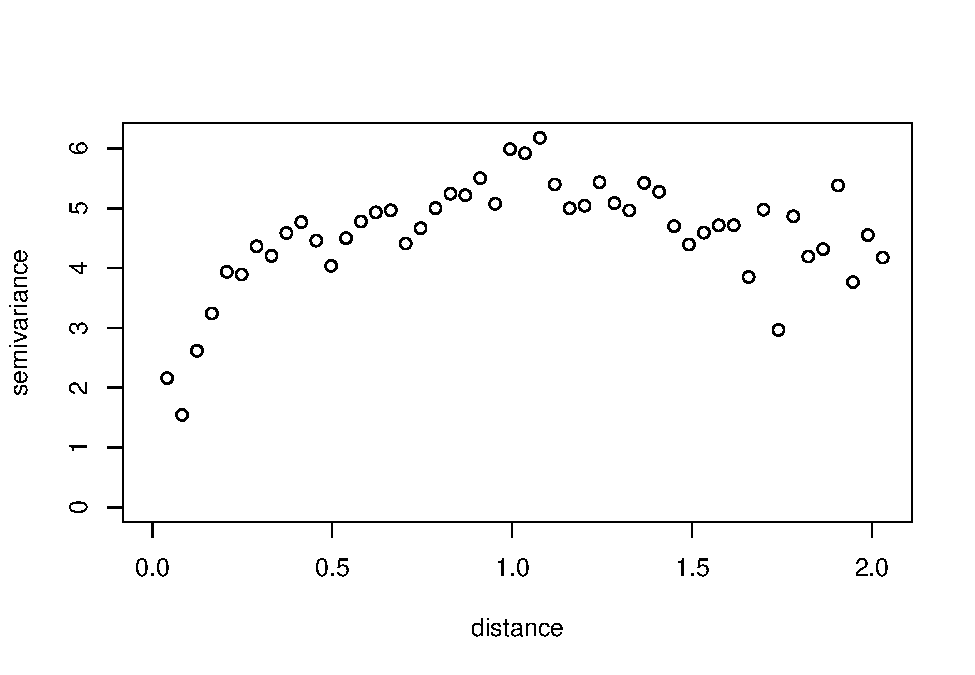
\includegraphics{Homework3_files/figure-latex/6x_vario-1.pdf}

\subsubsection{step 2: adjust paramters with
eyefit}\label{step-2-adjust-paramters-with-eyefit}

\begin{Shaded}
\begin{Highlighting}[]
\CommentTok{#adjust paramters with eyefit}
\KeywordTok{eyefit}\NormalTok{(myscps.vario,}\DataTypeTok{silent=}\OtherTok{TRUE}\NormalTok{)}
\end{Highlighting}
\end{Shaded}

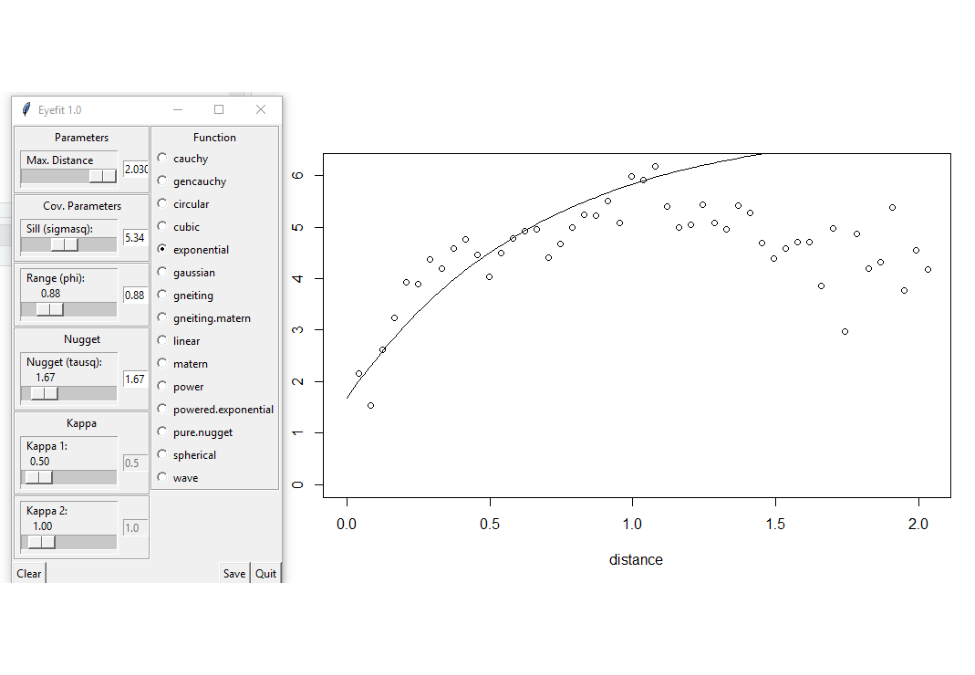
\includegraphics{Homework3_files/figure-latex/ex6_3dd-1.pdf}

\subsubsection{step 3: computing varfit}\label{step-3-computing-varfit}

According step 2 results, the following parameters should setting as
\(\sigma^2=5.34,\Phi=0.88\) and nugget=1.67. And \(exponential\) model
seems works fine.

\begin{Shaded}
\begin{Highlighting}[]
\NormalTok{fit.lgcatch<-}\StringTok{ }\KeywordTok{variofit}\NormalTok{(myscps.vario,}\DataTypeTok{cov.model=}\StringTok{"exponential"}\NormalTok{,}
                       \DataTypeTok{fix.nugget=}\OtherTok{FALSE}\NormalTok{, }\DataTypeTok{ini.cov.pars=}\KeywordTok{c}\NormalTok{(}\FloatTok{5.34}\NormalTok{,}\FloatTok{0.88}\NormalTok{), }
                       \DataTypeTok{nugget=}\FloatTok{1.67}\NormalTok{)}
\end{Highlighting}
\end{Shaded}

\begin{verbatim}
## variofit: covariance model used is exponential 
## variofit: weights used: npairs 
## variofit: minimisation function used: optim
\end{verbatim}

\begin{Shaded}
\begin{Highlighting}[]
\NormalTok{fit.lgcatch}
\end{Highlighting}
\end{Shaded}

\begin{verbatim}
## variofit: model parameters estimated by WLS (weighted least squares):
## covariance model is: exponential
## parameter estimates:
##   tausq sigmasq     phi 
##  0.3802  4.6326  0.1767 
## Practical Range with cor=0.05 for asymptotic range: 0.5292095
## 
## variofit: minimised weighted sum of squares = 2649.161
\end{verbatim}

\subsubsection{step 4: Kriging}\label{step-4-kriging}

According step 3 results, the following parameters should setting as
\(\sigma^2=4.6326,\Phi=0.1767\) and nugget=0.3802. Although the value
\(\Phi=0.1767\) is not making sense in the above results if we compare
to results from step 2, we will use this value to compute the last point
of the lgcatch data.

\begin{Shaded}
\begin{Highlighting}[]
\NormalTok{point<-}\KeywordTok{krige.conv}\NormalTok{(}\DataTypeTok{coords =}\NormalTok{ coords, }\DataTypeTok{data =}\NormalTok{ lgcatch,}\DataTypeTok{loc=}\KeywordTok{c}\NormalTok{(}\KeywordTok{length}\NormalTok{(lgcatch),}\DecValTok{1}\NormalTok{),}
                  \DataTypeTok{krige=}\KeywordTok{krige.control}\NormalTok{(}\DataTypeTok{cov.pars=}\KeywordTok{c}\NormalTok{(}\FloatTok{4.6326}\NormalTok{,}\FloatTok{0.1767}\NormalTok{),}
                                      \DataTypeTok{cov.model=}\StringTok{"exponential"}\NormalTok{,}
                                      \DataTypeTok{nugget=}\FloatTok{0.3802}\NormalTok{))}
\end{Highlighting}
\end{Shaded}

\begin{verbatim}
## krige.conv: model with constant mean
## krige.conv: Kriging performed using global neighbourhood
\end{verbatim}

\begin{Shaded}
\begin{Highlighting}[]
\NormalTok{point}
\end{Highlighting}
\end{Shaded}

\begin{verbatim}
## $predict
##     data 
## 2.644499 
## 
## $krige.var
## [1] 5.263914
## 
## $beta.est
##     beta 
## 2.644499 
## 
## $distribution
## [1] "normal"
## 
## $message
## [1] "krige.conv: Kriging performed using global neighbourhood"
## 
## $call
## krige.conv(coords = coords, data = lgcatch, locations = c(length(lgcatch), 
##     1), krige = krige.control(cov.pars = c(4.6326, 0.1767), cov.model = "exponential", 
##     nugget = 0.3802))
## 
## attr(,"sp.dim")
## [1] "2d"
## attr(,"prediction.locations")
## c(length(lgcatch), 1)
## attr(,"parent.env")
## <environment: R_GlobalEnv>
## attr(,"data.locations")
## coords
## attr(,"class")
## [1] "kriging"
\end{verbatim}

\begin{Shaded}
\begin{Highlighting}[]
\NormalTok{pred_low <-point}\OperatorTok{$}\NormalTok{predict }\OperatorTok{-}\StringTok{ }\DecValTok{2}\OperatorTok{*}\KeywordTok{sqrt}\NormalTok{(point}\OperatorTok{$}\NormalTok{krige.var)}
\NormalTok{pred_high <-point}\OperatorTok{$}\NormalTok{predict }\OperatorTok{+}\StringTok{ }\DecValTok{2}\OperatorTok{*}\KeywordTok{sqrt}\NormalTok{(point}\OperatorTok{$}\NormalTok{krige.var)}
\KeywordTok{print}\NormalTok{(}\KeywordTok{paste}\NormalTok{(}\StringTok{"The PI is between"}\NormalTok{,pred_low,}\StringTok{"and"}\NormalTok{,pred_high))}
\end{Highlighting}
\end{Shaded}

\begin{verbatim}
## [1] "The PI is between -1.94414491080096 and 7.23314348012374"
\end{verbatim}

\subsubsection{step 5: Summary Results}\label{step-5-summary-results}

As we can see from above, the predict and varirance are 2.64 and 5.26;
therefore, the PI with \(95\%\) confident is beteewn
\(2.64-2\times\sqrt{5.26}= -1.94\) and \(2.64+2\times\sqrt{5.26}=7.23\),
more accurate numbers have been printed above.

\section{Excerise 7}\label{excerise-7}

\subsubsection{step 1:load data and plot
variogram}\label{step-1load-data-and-plot-variogram-1}

\begin{Shaded}
\begin{Highlighting}[]
\NormalTok{url_coal <-}\StringTok{ "https://www.counterpointstat.com/uploads/1/1/9/3/119383887/coal.ash.txt"} 
\NormalTok{coalash <-}\StringTok{ }\KeywordTok{read.table}\NormalTok{(url_coal,}\DataTypeTok{header =}\NormalTok{ T)}


\NormalTok{coords_coal <-}\StringTok{ }\KeywordTok{as.matrix}\NormalTok{(coalash[,}\KeywordTok{c}\NormalTok{(}\StringTok{"x"}\NormalTok{,}\StringTok{"y"}\NormalTok{)]) }
\NormalTok{coal <-}\StringTok{ }\NormalTok{coalash}\OperatorTok{$}\NormalTok{coal}
\NormalTok{vario.coal <-}\StringTok{ }\KeywordTok{variog}\NormalTok{(}\DataTypeTok{coords =}\NormalTok{ coords_coal, }\DataTypeTok{data =}\NormalTok{ coal, }\DataTypeTok{uvec =}\NormalTok{ (}\KeywordTok{seq}\NormalTok{(}\DecValTok{0}\NormalTok{, }\DataTypeTok{length =}\NormalTok{ bins)))}
\end{Highlighting}
\end{Shaded}

\begin{verbatim}
## variog: computing omnidirectional variogram
\end{verbatim}

\begin{Shaded}
\begin{Highlighting}[]
\KeywordTok{plot}\NormalTok{(vario.coal)}
\end{Highlighting}
\end{Shaded}

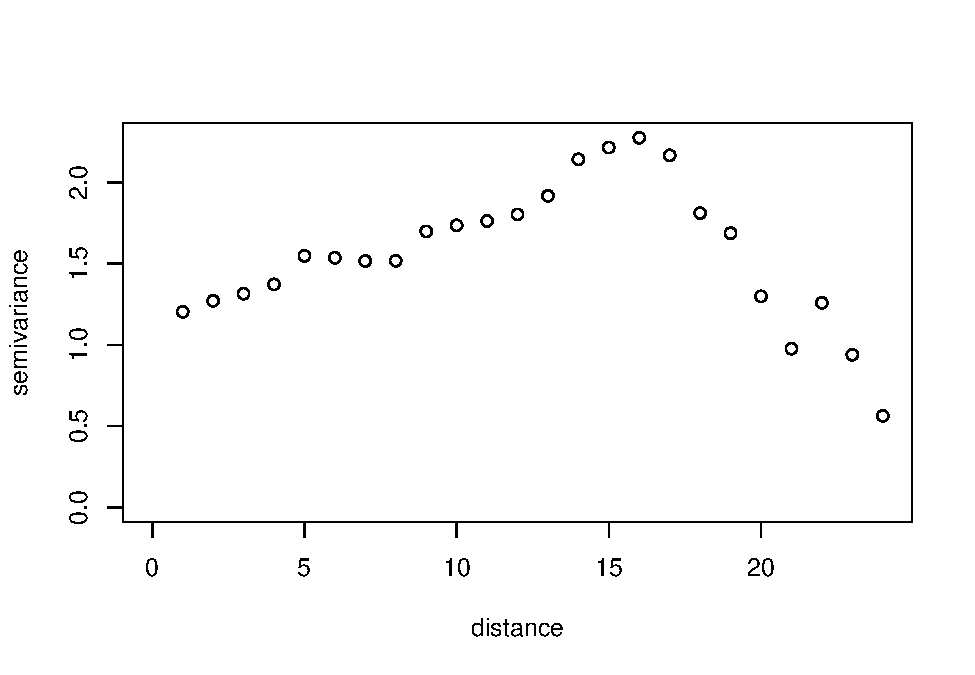
\includegraphics{Homework3_files/figure-latex/7x_vario-1.pdf}

\subsubsection{step 2: adjust paramters with
eyefit}\label{step-2-adjust-paramters-with-eyefit-1}

\begin{Shaded}
\begin{Highlighting}[]
\KeywordTok{eyefit}\NormalTok{(vario.coal ,}\DataTypeTok{silent=}\OtherTok{TRUE}\NormalTok{)}
\end{Highlighting}
\end{Shaded}

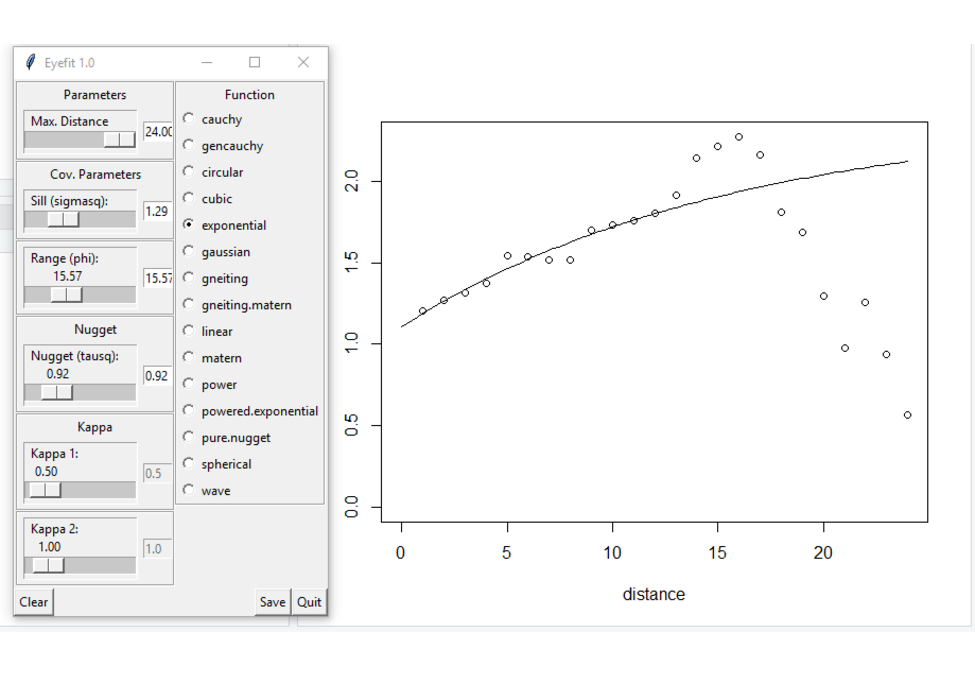
\includegraphics{Homework3_files/figure-latex/ex7_3dd-1.pdf}

\subsubsection{step 3: computing
varfit}\label{step-3-computing-varfit-1}

According step 2 results, the following parameters should setting as
\(\sigma^2=1.29,\Phi=15.57\) and nugget=0.92. However, the value shown
in eyefit results is a little strange, it may more make sense if we
choose about \(\frac{1}{17}\) base on variogram. In the following code,
let's try both values of \(\Phi\) and select the one produces more
accurate results in predicting \(\tau^2\) and \(\sigma^2\).

And \(exponential\) model seems works fine.

\begin{Shaded}
\begin{Highlighting}[]
\NormalTok{fit.coal<-}\StringTok{ }\KeywordTok{variofit}\NormalTok{(vario.coal,}\DataTypeTok{cov.model=}\StringTok{"exponential"}\NormalTok{,}
                    \DataTypeTok{fix.nugget=}\OtherTok{FALSE}\NormalTok{,}
                    \DataTypeTok{ini.cov.pars=}\KeywordTok{c}\NormalTok{(}\FloatTok{1.29}\NormalTok{,}\DecValTok{1}\OperatorTok{/}\DecValTok{17}\NormalTok{), }\DataTypeTok{nugget=}\FloatTok{0.92}\NormalTok{)}
\end{Highlighting}
\end{Shaded}

\begin{verbatim}
## variofit: covariance model used is exponential 
## variofit: weights used: npairs 
## variofit: minimisation function used: optim
\end{verbatim}

\begin{Shaded}
\begin{Highlighting}[]
\NormalTok{fit.coal}
\end{Highlighting}
\end{Shaded}

\begin{verbatim}
## variofit: model parameters estimated by WLS (weighted least squares):
## covariance model is: exponential
## parameter estimates:
##   tausq sigmasq     phi 
##  0.6712  0.9437  2.0996 
## Practical Range with cor=0.05 for asymptotic range: 6.289926
## 
## variofit: minimised weighted sum of squares = 1183.811
\end{verbatim}

\begin{Shaded}
\begin{Highlighting}[]
\NormalTok{fit.coal<-}\StringTok{ }\KeywordTok{variofit}\NormalTok{(vario.coal,}\DataTypeTok{cov.model=}\StringTok{"exponential"}\NormalTok{,}
                    \DataTypeTok{fix.nugget=}\OtherTok{FALSE}\NormalTok{,}
                    \DataTypeTok{ini.cov.pars=}\KeywordTok{c}\NormalTok{(}\FloatTok{1.29}\NormalTok{,}\FloatTok{15.57}\NormalTok{), }\DataTypeTok{nugget=}\FloatTok{0.92}\NormalTok{)}
\end{Highlighting}
\end{Shaded}

\begin{verbatim}
## variofit: covariance model used is exponential 
## variofit: weights used: npairs 
## variofit: minimisation function used: optim
\end{verbatim}

\begin{Shaded}
\begin{Highlighting}[]
\NormalTok{fit.coal}
\end{Highlighting}
\end{Shaded}

\begin{verbatim}
## variofit: model parameters estimated by WLS (weighted least squares):
## covariance model is: exponential
## parameter estimates:
##   tausq sigmasq     phi 
##  1.0372  1.2026 11.1435 
## Practical Range with cor=0.05 for asymptotic range: 33.38281
## 
## variofit: minimised weighted sum of squares = 498.1197
\end{verbatim}

\subsubsection{step 4: Kriging
Prediction}\label{step-4-kriging-prediction}

According step 3 results, Even though set \(\phi=\frac{1}{17}\) is make
more sense but the model can produce more accurate values of \(\tau^2\)
and \(\sigma^2\) by setting \(\phi=15.57\). Therefore, we will adopt the
results from the second option. And the following parameters should
setting as \(\sigma^2=1.2026,\Phi=11.1435\) and \(\tau^2=1.0372\).

\begin{Shaded}
\begin{Highlighting}[]
\NormalTok{point<-}\KeywordTok{krige.conv}\NormalTok{(}\DataTypeTok{coords =}\NormalTok{ coords_coal, }\DataTypeTok{data =}\NormalTok{ coal,}\DataTypeTok{loc=}\KeywordTok{c}\NormalTok{(}\KeywordTok{length}\NormalTok{(coal),}\DecValTok{1}\NormalTok{),}
                  \DataTypeTok{krige=}\KeywordTok{krige.control}\NormalTok{(}\DataTypeTok{cov.pars=}\KeywordTok{c}\NormalTok{(}\FloatTok{1.2026}\NormalTok{,}\FloatTok{11.1435}\NormalTok{),}\DataTypeTok{cov.model=}\StringTok{"exponential"}\NormalTok{,}\DataTypeTok{nugget=}\FloatTok{1.0372}\NormalTok{))}
\end{Highlighting}
\end{Shaded}

\begin{verbatim}
## krige.conv: model with constant mean
## krige.conv: Kriging performed using global neighbourhood
\end{verbatim}

\begin{Shaded}
\begin{Highlighting}[]
\NormalTok{point}
\end{Highlighting}
\end{Shaded}

\begin{verbatim}
## $predict
##     data 
## 9.663041 
## 
## $krige.var
## [1] 2.761329
## 
## $beta.est
##     beta 
## 9.663041 
## 
## $distribution
## [1] "normal"
## 
## $message
## [1] "krige.conv: Kriging performed using global neighbourhood"
## 
## $call
## krige.conv(coords = coords_coal, data = coal, locations = c(length(coal), 
##     1), krige = krige.control(cov.pars = c(1.2026, 11.1435), 
##     cov.model = "exponential", nugget = 1.0372))
## 
## attr(,"sp.dim")
## [1] "2d"
## attr(,"prediction.locations")
## c(length(coal), 1)
## attr(,"parent.env")
## <environment: R_GlobalEnv>
## attr(,"data.locations")
## coords_coal
## attr(,"class")
## [1] "kriging"
\end{verbatim}

\begin{Shaded}
\begin{Highlighting}[]
\NormalTok{pred_low <-point}\OperatorTok{$}\NormalTok{predict }\OperatorTok{-}\StringTok{ }\DecValTok{2}\OperatorTok{*}\KeywordTok{sqrt}\NormalTok{(point}\OperatorTok{$}\NormalTok{krige.var)}
\NormalTok{pred_high <-point}\OperatorTok{$}\NormalTok{predict }\OperatorTok{+}\StringTok{ }\DecValTok{2}\OperatorTok{*}\KeywordTok{sqrt}\NormalTok{(point}\OperatorTok{$}\NormalTok{krige.var)}
\KeywordTok{print}\NormalTok{(}\KeywordTok{paste}\NormalTok{(}\StringTok{"The PI is between"}\NormalTok{,pred_low,}\StringTok{"and"}\NormalTok{,pred_high))}
\end{Highlighting}
\end{Shaded}

\begin{verbatim}
## [1] "The PI is between 6.33959120662333 and 12.9864901385506"
\end{verbatim}

\subsubsection{step 5: Summary Results}\label{step-5-summary-results-1}

As we can see from above, the predict and varirance are 9.66 and 2.76;
therefore, the PI with \(95\%\) confident is beteewn
\(9.66-2\times\sqrt{2.76}= 6.34\) and \(9.66+2\times\sqrt{2.76}=12.98\),
more accurate numbers have been printed above.

\section{Using Matrix Method}\label{using-matrix-method}

\section{Exercise 6}\label{exercise-6}

Given same previous work and choose paramters as below:

\begin{Shaded}
\begin{Highlighting}[]
\CommentTok{# assign the coords to given_coords except last row}

\NormalTok{given_coords <-}\StringTok{ }\NormalTok{coords[}\DecValTok{1}\OperatorTok{:}\KeywordTok{dim}\NormalTok{(coords)[}\DecValTok{1}\NormalTok{]}\OperatorTok{-}\DecValTok{1}\NormalTok{,]}
\NormalTok{myscallops.covmat<-}\KeywordTok{varcov.spatial}\NormalTok{(}\DataTypeTok{coords =}\NormalTok{ given_coords,}
                                  \DataTypeTok{cov.model =} \StringTok{"exponential"}\NormalTok{, }
                                 \DataTypeTok{nugget =} \FloatTok{1.67}\NormalTok{,}
                                 \DataTypeTok{cov.pars =} \KeywordTok{c}\NormalTok{(}\FloatTok{5.34}\NormalTok{,}\FloatTok{0.88}\NormalTok{))}
\CommentTok{# just print myscallops.covmat will be too long!}
\CommentTok{# myscallops.covmat}
\CommentTok{# setup covariance matrix with point for prediction}
\NormalTok{gamma_all<-}\KeywordTok{varcov.spatial}\NormalTok{(}\DataTypeTok{coords =}\NormalTok{ coords,}
                           \DataTypeTok{cov.model =} \StringTok{"exponential"}\NormalTok{, }
                           \DataTypeTok{nugget =} \FloatTok{1.67}\NormalTok{,}
                           \DataTypeTok{cov.pars =} \KeywordTok{c}\NormalTok{(}\FloatTok{5.34}\NormalTok{,}\FloatTok{0.88}\NormalTok{))}
\CommentTok{# we are interested in last column}
\NormalTok{gamma <-}\StringTok{ }\NormalTok{gamma_all}\OperatorTok{$}\NormalTok{varcov[,}\KeywordTok{ncol}\NormalTok{(gamma_all}\OperatorTok{$}\NormalTok{varcov)]}
\NormalTok{cov <-}\StringTok{ }\NormalTok{gamma[}\KeywordTok{length}\NormalTok{(gamma)]}
\NormalTok{gamma <-}\StringTok{ }\NormalTok{gamma[}\OperatorTok{-}\KeywordTok{length}\NormalTok{(gamma)]}

\NormalTok{z <-}\StringTok{ }\NormalTok{lgcatch[}\OperatorTok{-}\KeywordTok{length}\NormalTok{(lgcatch)]}
\NormalTok{mu <-}\StringTok{ }\KeywordTok{mean}\NormalTok{(z)}
\NormalTok{m <-}\StringTok{ }\KeywordTok{rep}\NormalTok{(mu, }\KeywordTok{length}\NormalTok{(z))}
\NormalTok{m <-}\StringTok{ }\KeywordTok{matrix}\NormalTok{(m,}\DataTypeTok{nrow=}\KeywordTok{length}\NormalTok{(z),}\DataTypeTok{ncol=}\DecValTok{1}\NormalTok{)}
\NormalTok{z <-}\StringTok{ }\KeywordTok{matrix}\NormalTok{(z,}\DataTypeTok{nrow=}\KeywordTok{length}\NormalTok{(z),}\DataTypeTok{ncol=}\DecValTok{1}\NormalTok{)}


\NormalTok{y_pred<-}\StringTok{ }\NormalTok{mu }\OperatorTok{+}\KeywordTok{t}\NormalTok{(gamma)}\OperatorTok\KeywordTok{solve}\NormalTok{(myscallops.covmat}\OperatorTok{$}\NormalTok{varcov)}\OperatorTok\NormalTok{(z}\OperatorTok{-}\NormalTok{m)}
\NormalTok{y_pred}
\end{Highlighting}
\end{Shaded}

\begin{verbatim}
##          [,1]
## [1,] 2.960819
\end{verbatim}

\begin{Shaded}
\begin{Highlighting}[]
\CommentTok{# now compute variance}

\NormalTok{cov}
\end{Highlighting}
\end{Shaded}

\begin{verbatim}
## [1] 7.01
\end{verbatim}

\begin{Shaded}
\begin{Highlighting}[]
\NormalTok{var_pred<-cov }\OperatorTok{-}\KeywordTok{t}\NormalTok{(gamma)}\OperatorTok\KeywordTok{solve}\NormalTok{(myscallops.covmat}\OperatorTok{$}\NormalTok{varcov)}\OperatorTok\NormalTok{gamma}
\NormalTok{var_pred}
\end{Highlighting}
\end{Shaded}

\begin{verbatim}
##          [,1]
## [1,] 2.369833
\end{verbatim}

\begin{Shaded}
\begin{Highlighting}[]
\NormalTok{pred_low <-}\StringTok{ }\NormalTok{y_pred }\OperatorTok{-}\StringTok{ }\DecValTok{2}\OperatorTok{*}\KeywordTok{sqrt}\NormalTok{(var_pred)}
\NormalTok{pred_high <-}\StringTok{ }\NormalTok{y_pred }\OperatorTok{+}\StringTok{ }\DecValTok{2}\OperatorTok{*}\KeywordTok{sqrt}\NormalTok{(var_pred)}
\KeywordTok{print}\NormalTok{(}\KeywordTok{paste}\NormalTok{(}\StringTok{"The PI is between"}\NormalTok{,pred_low,}\StringTok{"and"}\NormalTok{,pred_high))}
\end{Highlighting}
\end{Shaded}

\begin{verbatim}
## [1] "The PI is between -0.11803299551682 and 6.03967116464465"
\end{verbatim}

As we can see, from above results, the matrix method results is almost
the same as the API function results.

\section{Exercise 7}\label{exercise-7}

Given same previous work and choose paramters as below:

\begin{Shaded}
\begin{Highlighting}[]
\CommentTok{# assign the coords to given_coords except last row}

\NormalTok{given_coords <-}\StringTok{ }\NormalTok{coords_coal[}\DecValTok{1}\OperatorTok{:}\KeywordTok{dim}\NormalTok{(coords_coal)[}\DecValTok{1}\NormalTok{]}\OperatorTok{-}\DecValTok{1}\NormalTok{,]}
\NormalTok{coal.covmat<-}\KeywordTok{varcov.spatial}\NormalTok{(}\DataTypeTok{coords =}\NormalTok{ given_coords,}
                                  \DataTypeTok{cov.model =} \StringTok{"exponential"}\NormalTok{, }
                                 \DataTypeTok{nugget =} \FloatTok{1.0372}\NormalTok{,}
                                 \DataTypeTok{cov.pars =} \KeywordTok{c}\NormalTok{(}\FloatTok{1.2026}\NormalTok{,}\FloatTok{11.1435}\NormalTok{))}
\CommentTok{# just print myscallops.covmat will be too long!}
\CommentTok{# myscallops.covmat}
\CommentTok{# setup covariance matrix with point for prediction}
\NormalTok{gamma_all<-}\KeywordTok{varcov.spatial}\NormalTok{(}\DataTypeTok{coords =}\NormalTok{ coords_coal,}
                           \DataTypeTok{cov.model =} \StringTok{"exponential"}\NormalTok{, }
                           \DataTypeTok{nugget =} \FloatTok{1.0372}\NormalTok{,}
                           \DataTypeTok{cov.pars =} \KeywordTok{c}\NormalTok{(}\FloatTok{1.2026}\NormalTok{,}\FloatTok{11.1435}\NormalTok{))}
\CommentTok{# we are interested in last column}
\NormalTok{gamma <-}\StringTok{ }\NormalTok{gamma_all}\OperatorTok{$}\NormalTok{varcov[,}\KeywordTok{ncol}\NormalTok{(gamma_all}\OperatorTok{$}\NormalTok{varcov)]}
\NormalTok{cov <-}\StringTok{ }\NormalTok{gamma[}\KeywordTok{length}\NormalTok{(gamma)]}
\NormalTok{gamma <-}\StringTok{ }\NormalTok{gamma[}\OperatorTok{-}\KeywordTok{length}\NormalTok{(gamma)]}

\NormalTok{z <-}\StringTok{ }\NormalTok{coal[}\OperatorTok{-}\KeywordTok{length}\NormalTok{(coal)]}
\NormalTok{mu <-}\StringTok{ }\KeywordTok{mean}\NormalTok{(z)}
\NormalTok{m <-}\StringTok{ }\KeywordTok{rep}\NormalTok{(mu, }\KeywordTok{length}\NormalTok{(z))}
\NormalTok{m <-}\StringTok{ }\KeywordTok{matrix}\NormalTok{(m,}\DataTypeTok{nrow=}\KeywordTok{length}\NormalTok{(z),}\DataTypeTok{ncol=}\DecValTok{1}\NormalTok{)}
\NormalTok{z <-}\StringTok{ }\KeywordTok{matrix}\NormalTok{(z,}\DataTypeTok{nrow=}\KeywordTok{length}\NormalTok{(z),}\DataTypeTok{ncol=}\DecValTok{1}\NormalTok{)}


\NormalTok{y_pred<-}\StringTok{ }\NormalTok{mu }\OperatorTok{+}\KeywordTok{t}\NormalTok{(gamma)}\OperatorTok\KeywordTok{solve}\NormalTok{(coal.covmat}\OperatorTok{$}\NormalTok{varcov)}\OperatorTok\NormalTok{(z}\OperatorTok{-}\NormalTok{m)}
\NormalTok{y_pred}
\end{Highlighting}
\end{Shaded}

\begin{verbatim}
##          [,1]
## [1,] 8.612182
\end{verbatim}

\begin{Shaded}
\begin{Highlighting}[]
\CommentTok{# now compute variance}

\NormalTok{cov}
\end{Highlighting}
\end{Shaded}

\begin{verbatim}
## [1] 2.2398
\end{verbatim}

\begin{Shaded}
\begin{Highlighting}[]
\NormalTok{var_pred<-cov }\OperatorTok{-}\KeywordTok{t}\NormalTok{(gamma)}\OperatorTok\KeywordTok{solve}\NormalTok{(coal.covmat}\OperatorTok{$}\NormalTok{varcov)}\OperatorTok\NormalTok{gamma}
\NormalTok{var_pred}
\end{Highlighting}
\end{Shaded}

\begin{verbatim}
##          [,1]
## [1,] 1.391571
\end{verbatim}

\begin{Shaded}
\begin{Highlighting}[]
\NormalTok{pred_low <-}\StringTok{ }\NormalTok{y_pred }\OperatorTok{-}\StringTok{ }\DecValTok{2}\OperatorTok{*}\KeywordTok{sqrt}\NormalTok{(var_pred)}
\NormalTok{pred_high <-}\StringTok{ }\NormalTok{y_pred }\OperatorTok{+}\StringTok{ }\DecValTok{2}\OperatorTok{*}\KeywordTok{sqrt}\NormalTok{(var_pred)}
\KeywordTok{print}\NormalTok{(}\KeywordTok{paste}\NormalTok{(}\StringTok{"The PI is between"}\NormalTok{,pred_low,}\StringTok{"and"}\NormalTok{,pred_high))}
\end{Highlighting}
\end{Shaded}

\begin{verbatim}
## [1] "The PI is between 6.25288475730364 and 10.971479547674"
\end{verbatim}

As we can see, from above results, the matrix method results is clost to
the API function results to some extend.


\end{document}
